\documentclass{article}
\usepackage{amsmath}
\usepackage{amssymb}
\usepackage{graphicx}
\usepackage{hyperref}
\usepackage[version=4]{mhchem}

\title{Problem 9}
\date{}

\begin{document}
\maketitle

\section*{Problem}
(2012 Mathcounts State Sprint 30) In rectangle \(A B C D\), shown here, point \(M\) is the midpoint of side \(B C\), and point \(N\) lies on \(C D\) such that \(D N: N C=1: 4\). Segment \(B N\) intersects \(A M\) and \(A C\) at points \(R\) and \(S\), respectively. If \(N S: S R: R B=x: y: z\), where \(x, y\) and \(z\) are positive integers, what is the minimum possible value of \(x+y+z\) ?\\
\centering
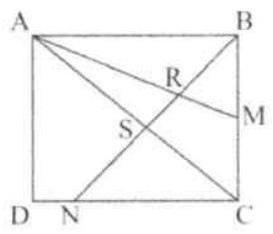
\includegraphics[width=\textwidth]{images/problem_image_1.jpg}

\section*{Solution}
126.
Draw \(M E / / N C\) to meet \(N B\) at \(E . \triangle A B S \sim \triangle C N S, \triangle A B R \sim \triangle M E R\). Since \(D N: N C\) \(=1: 4, N C=\frac{4}{5} A B\). So \(E M=\frac{1}{2} N C=\frac{1}{2} \times \frac{4}{5} A B=\frac{2}{5} A B\).\\
So \(B E=E N=\frac{x+y+z}{2}\), and \(E R=E B-R B=\frac{x+y+z}{2}-z=\frac{x+y-z}{2}\).\\
\(\frac{A B}{N C}=\frac{B S}{N S}=\frac{5}{4} \quad \Rightarrow \quad \frac{y+z}{x}=\frac{5}{4} \quad \Rightarrow \quad 5 x=4 y+4 z\)\\
\(\frac{A B}{E M}=\frac{B R}{E R}=\frac{5}{2} \quad \Rightarrow \quad \frac{z}{\frac{x+y-z}{2}}=\frac{5}{2} \quad \Rightarrow\)

\[
4 z=5 x+5 y-5 z \quad \Rightarrow \quad 5 x+5 y=9 z
\]

Solving the system of equations (1) and (2): \(\frac{x}{y}=\frac{56}{25}\), and \(\frac{y}{z}=\frac{5}{9}\).\\
Thus \(x: y: z=56: 25: 45\). The smallest value of \(x+y+z\) is \(56+25+45=126\).\\
\centering
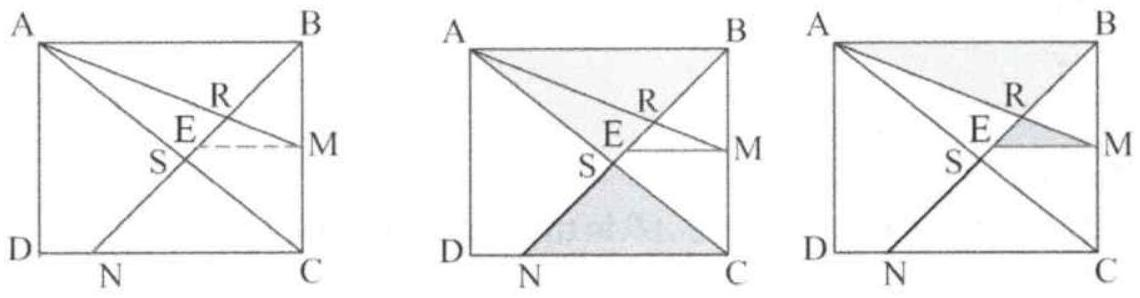
\includegraphics[width=\textwidth]{images/reasoning_image_1.jpg}

\end{document}
